% ============================================================
%  يُترجَم بـ XeLaTeX  (في Overleaf: Menu → Compiler → XeLaTeX)
%  الخط: Amiri (متوفر في Overleaf، أو حمّله من github.com/aliftype/amiri)
% ============================================================
\documentclass[12pt,a4paper]{article}
\usepackage[a4paper,margin=1.7cm,top=2.3cm,bottom=2.9cm,headheight=15pt,footskip=1.5cm]{geometry}
\usepackage{amsmath,amssymb}
\usepackage{icomma}
\usepackage[english,bidi=default,layout=lists]{babel}
\babelprovide[import,main]{arabic}
\babelfont{rm}[Scale=1.08]{Amiri}
\babelfont{sf}[Scale=1.08]{Amiri}
\usepackage[most]{tcolorbox}
\usepackage{tikz}
\usetikzlibrary{arrows.meta,calc,shadings}
\usepackage{array}
\usepackage{colortbl}
\usepackage{fancyhdr}
\usepackage{titlesec}
\usepackage{enumitem}
\usepackage{collcell}
\usepackage{needspace}
\usepackage{etoolbox}
\newcolumntype{C}{>{\collectcell\ar}c<{\endcollectcell}}
\pretocmd{\section}{\Needspace{15\baselineskip}}{}{}
\pretocmd{\subsection}{\Needspace{11\baselineskip}}{}{}

\definecolor{cDef}{HTML}{1F4E9C}
\definecolor{cThm}{HTML}{B3261E}
\definecolor{cRem}{HTML}{2E7D32}
\definecolor{cEx}{HTML}{C76B00}
\definecolor{cMeth}{HTML}{6A1B9A}
\definecolor{cSol}{HTML}{00695C}
\definecolor{cSec}{HTML}{1F3A68}

\titleformat{\section}{\Large\bfseries\color{cSec}}{\thesection.}{0.6em}{}[{\color{cSec!60}\titlerule[1pt]}]
\titleformat{\subsection}{\large\bfseries\color{cThm!85!black}}{\thesubsection.}{0.5em}{}
\titlespacing*{\section}{0pt}{14pt}{8pt}
\titlespacing*{\subsection}{0pt}{10pt}{5pt}
\setlength{\parindent}{0pt}
\setlength{\parskip}{4pt}
\setlist{itemsep=2pt,topsep=3pt}

\newtcolorbox{arbox}[3][]{enhanced,
  colback=#2!5,colframe=#2!80!black,arc=2mm,boxrule=0.8pt,
  left=6pt,right=6pt,top=8pt,bottom=5pt,
  fonttitle=\bfseries,coltitle=white,
  title={\foreignlanguage{arabic}{#3}},
  attach boxed title to top right={xshift=-5mm,yshift=-3mm},
  boxed title style={colback=#2!80!black,arc=1.5mm,boxrule=0pt},
  before upper={\selectlanguage{arabic}},
  before skip=8pt,after skip=8pt,breakable,#1}
\newenvironment{BOX}[2]{\begin{otherlanguage}{english}\begin{arbox}{#1}{#2}}{\end{arbox}\end{otherlanguage}}
\newenvironment{tarif}[1][تعريف]{\begin{BOX}{cDef}{#1}}{\end{BOX}}
\newenvironment{khassia}[1][خاصية]{\begin{BOX}{cThm}{#1}}{\end{BOX}}
\newenvironment{molahada}[1][ملاحظة]{\begin{BOX}{cRem}{#1}}{\end{BOX}}
\newenvironment{mithal}[1][مثال]{\begin{BOX}{cEx}{#1}}{\end{BOX}}
\newenvironment{tariqa}[1][طريقة]{\begin{BOX}{cMeth}{#1}}{\end{BOX}}

\newcounter{exo}
\newenvironment{tamrin}[1]{\stepcounter{exo}\begin{BOX}{cSec}{التمرين \theexo: #1}}{\end{BOX}}
\newenvironment{hal}{\Needspace{12\baselineskip}\begin{otherlanguage}{english}\begin{arbox}[breakable]{cSol}{حل التمرين \theexo}}{\end{arbox}\end{otherlanguage}}

\newenvironment{LTR}{\begin{otherlanguage}{english}}{\end{otherlanguage}}
\newcommand{\ar}[1]{\foreignlanguage{arabic}{#1}}

\renewcommand{\dots}{\mathinner{\ldotp\ldotp\ldotp}}
\renewcommand{\ldots}{\mathinner{\ldotp\ldotp\ldotp}}
\renewcommand{\cdots}{\mathinner{\cdotp\cdotp\cdotp}}
\newcommand{\N}{\mathbb{N}}
\newcommand{\Z}{\mathbb{Z}}
\newcommand{\D}{\mathbb{D}}
\newcommand{\Q}{\mathbb{Q}}
\newcommand{\R}{\mathbb{R}}
\newcommand{\pgcd}{\operatorname{PGCD}}
\newcommand{\ppcm}{\operatorname{PPCM}}

% \NLseg{a}{b}{[}{]} ; \NLright{a}{[} ; \NLleft{b}{]}  (interval on a number line)
\newcommand{\NLseg}[4]{\begin{LTR}\begin{tikzpicture}[baseline=-0.6ex]
 \draw[-{Stealth[length=2mm]},gray!70](0,0)--(3.4,0);
 \draw[line width=2pt,cThm!80!black](0.7,0)--(2.7,0);
 \node[cThm!80!black,font=\LARGE] at (0.7,0){$#3$};
 \node[cThm!80!black,font=\LARGE] at (2.7,0){$#4$};
 \node[below=3pt,font=\footnotesize] at (0.7,0){$#1$};
 \node[below=3pt,font=\footnotesize] at (2.7,0){$#2$};
\end{tikzpicture}\end{LTR}}
\newcommand{\NLright}[2]{\begin{LTR}\begin{tikzpicture}[baseline=-0.6ex]
 \draw[-{Stealth[length=2mm]},gray!70](0,0)--(3.4,0);
 \draw[line width=2pt,cThm!80!black](1.3,0)--(3.3,0);
 \node[cThm!80!black,font=\LARGE] at (1.3,0){$#2$};
 \node[below=3pt,font=\footnotesize] at (1.3,0){$#1$};
\end{tikzpicture}\end{LTR}}
\newcommand{\NLleft}[2]{\begin{LTR}\begin{tikzpicture}[baseline=-0.6ex]
 \draw[-{Stealth[length=2mm]},gray!70](0,0)--(3.4,0);
 \draw[line width=2pt,cThm!80!black](0.05,0)--(2.1,0);
 \node[cThm!80!black,font=\LARGE] at (2.1,0){$#2$};
 \node[below=3pt,font=\footnotesize] at (2.1,0){$#1$};
\end{tikzpicture}\end{LTR}}

% ---------- social-media icons (pure TikZ) ----------
\definecolor{cFB}{HTML}{1877F2}
\definecolor{cTG}{HTML}{229ED9}
\definecolor{cIG1}{HTML}{FEDA75}
\definecolor{cIG2}{HTML}{D62976}
\definecolor{cIG3}{HTML}{4F5BD5}
\newcommand{\fbicon}{\begin{LTR}\begin{tikzpicture}[baseline=-0.75ex,x=1em,y=1em]
 \fill[cFB] (0,0) circle (0.55);
 \node[white,inner sep=0,font=\usefont{TU}{lmss}{bx}{n}\small] at (0.04,-0.02) {f};
\end{tikzpicture}\end{LTR}}
\newcommand{\igicon}{\begin{LTR}
\begin{tikzpicture}[baseline=-0.75ex,x=1em,y=1em]
 \shade[lower left=cIG1,lower right=cIG2,upper left=cIG2,upper right=cIG3,rounded corners=0.28em] (-0.55,-0.55) rectangle (0.55,0.55);
 \draw[white,line width=0.09em,rounded corners=0.18em] (-0.36,-0.36) rectangle (0.36,0.36);
 \draw[white,line width=0.09em] (0,0) circle (0.17);
 \fill[white] (0.22,0.22) circle (0.05);
\end{tikzpicture}\end{LTR}}
\newcommand{\tgicon}{\begin{LTR}
\begin{tikzpicture}[baseline=-0.75ex,x=1em,y=1em]
 \fill[cTG] (0,0) circle (0.55);
 \fill[white] (-0.33,0.0) -- (0.32,0.27) -- (0.2,-0.3) -- (0.0,-0.15) -- (-0.08,-0.28) -- (-0.08,-0.08) -- cycle;
 \fill[cTG!70!black] (-0.08,-0.08) -- (0.25,0.2) -- (0.0,-0.15) -- (-0.08,-0.28) -- cycle;
\end{tikzpicture}\end{LTR}}
% page number: black box, white two-digit number, at the right of the social row
\newcommand{\PageBox}{\begin{LTR}\tikz[baseline=(p.base)]\node[fill=black,text=white,inner sep=2.5pt,minimum width=1.6em,minimum height=1.3em,font=\usefont{TU}{lmss}{bx}{n}\small](p){\ifnum\value{page}<10 0\fi\arabic{page}};\end{LTR}}
% visual left-to-right order: Telegram | Instagram | Facebook | page box
\newcommand{\SocialRow}{\begin{otherlanguage}{english}%
 \ar{\textbf{الأستاذ سوايسية هشام للرياضيات}}\ \tgicon\hfill
 \textbf{prof\_hicham\_math}\ \igicon\hfill
 \ar{\textbf{الأستاذ سوايسية هشام للرياضيات}}\ \fbicon\hspace{2.2em}\PageBox\end{otherlanguage}}

\pagestyle{fancy}
\fancyhf{}
\renewcommand{\headrulewidth}{0.6pt}
\renewcommand{\footrulewidth}{0.4pt}
% \SetHeader{right head: document title}{left head: level -- stream}
\newcommand{\SetHeader}[2]{%
 \fancyhead[C]{\parbox{\textwidth}{\ar{#1\hfill #2}}}%
 \fancyfoot[C]{\parbox{\textwidth}{\small\SocialRow}}}
\usepackage{tkz-tab}
\usepackage{multicol}
% variation / sign table (LTR)
\newenvironment{TAB}{\par\begin{center}\begin{LTR}\begin{tikzpicture}[scale=0.95,every node/.style={font=\small}]}{\end{tikzpicture}\end{LTR}\end{center}}
% grid + axes, clipped: \begin{GR}{xmin}{xmax}{ymin}{ymax}{unit cm}
\newenvironment{GR}[5]{\par\begin{center}\begin{LTR}\begin{tikzpicture}[x=#5cm,y=#5cm,font=\footnotesize]
 \draw[gray!25,very thin] (#1,#3) grid (#2,#4);
 \draw[-{Stealth[length=2mm]}] (#1,0)--(#2+0.3,0) node[below left]{$x$};
 \draw[-{Stealth[length=2mm]}] (0,#3)--(0,#4+0.3) node[below left]{$y$};
 \node[below left] at (0,0){$O$};
 \begin{scope}\clip (#1,#3) rectangle (#2,#4);}
{\end{scope}\end{tikzpicture}\end{LTR}\end{center}}
\newcommand{\Ticks}[2]{\foreach \t in {#1} \node[below,font=\scriptsize] at (\t,0){$\t$}; \foreach \t in {#2} \node[left,font=\scriptsize] at (0,\t){$\t$};}
\newcommand{\bx}[1]{\ensuremath{\colorbox{cDef!12}{$\displaystyle #1$}}}
\newcommand{\TwoCol}[4]{\par\begin{LTR}\noindent\begin{minipage}[t]{#1\textwidth}\selectlanguage{arabic}#2\end{minipage}\hfill\begin{minipage}[t]{#3\textwidth}\selectlanguage{arabic}#4\end{minipage}\end{LTR}\par}
\newcommand{\RL}[4]{\TwoCol{#3}{#4}{#1}{#2}}  % \RL{w1}{right content}{w2}{left content}
\newcommand{\ok}{$\textcolor{cRem}{\checkmark}$}
\newcommand{\limn}{\displaystyle\lim_{n\to+\infty}}
% sub-questions, each on its own line
\newenvironment{sq}{\begin{itemize}[leftmargin=2.4em,itemsep=3pt]}{\end{itemize}}
\newcommand{\qa}{\item[(أ)]}\newcommand{\qb}{\item[(ب)]}\newcommand{\qc}{\item[(جـ)]}\newcommand{\qd}{\item[(د)]}\newcommand{\qe}{\item[(هـ)]}
\newcommand{\pa}{\par\smallskip\textbf{(أ)} }\newcommand{\pb}{\par\smallskip\textbf{(ب)} }\newcommand{\pc}{\par\smallskip\textbf{(جـ)} }\newcommand{\pd}{\par\smallskip\textbf{(د)} }\newcommand{\pe}{\par\smallskip\textbf{(هـ)} }
\newcommand{\QQ}[1]{\par\smallskip\textbf{#1.} }
\newenvironment{tmr}{\stepcounter{exo}\begin{BOX}{cSec}{تمرين محلول \theexo}}{\end{BOX}}
\newcommand{\ABC}[3]{\\[2pt]\begin{tabular}{p{0.28\textwidth}p{0.28\textwidth}p{0.28\textwidth}}(جـ) \ #3 & (ب) \ #2 & (أ) \ #1\end{tabular}}
\pretocmd{\section}{\Needspace{24\baselineskip}}{}{}
\newtcbox{\bxtbox}{on line,colback=cDef!12,colframe=cDef!12,boxrule=0pt,arc=1pt,boxsep=0pt,left=2pt,right=2pt,top=1pt,bottom=1pt}
\newcommand{\bxt}[1]{\foreignlanguage{english}{\bxtbox{\ar{#1}}}}
\usepackage{longtable}
\setlength{\LTpre}{4pt}\setlength{\LTpost}{0pt}
\newcommand{\Phase}[1]{\textbf{#1}}
\newcommand{\Fld}[2]{\textbf{#1:}\ #2}
% رأس المذكرة على نمط النموذج: إطار بعنوان «مذكرة رقم»، معلومات الحصة، ثم إطار الكفاءات
\newcommand{\ModhHead}[9]{%
\begin{LTR}
\begin{tcolorbox}[enhanced,colback=white,colframe=cThm!85!black,arc=4mm,boxrule=1pt,top=14pt,bottom=6pt,left=8pt,right=8pt,
 overlay={\node[fill=cThm!85!black,text=white,rounded corners=3mm,inner xsep=14pt,inner ysep=4pt,font=\large\bfseries] at ([yshift=0pt]frame.north){\ar{مذكرة رقم #1}};},
 before upper={\selectlanguage{arabic}}]
\begin{tabular}{@{}p{0.4\linewidth}p{0.55\linewidth}@{}}
\Fld{المستوى}{#2} & \Fld{الثانوية}{\dotfill}\\[3pt]
\Fld{المادة}{رياضيات} & \Fld{ميدان التعلم}{#3}\\[3pt]
\Fld{المدة}{#5} & \Fld{الوحدة التعلمية}{#4}\\[3pt]
\Fld{الأستاذ}{\dotfill} & \Fld{المحتوى المعرفي}{#6}\\
\end{tabular}
\end{tcolorbox}
\begin{tcolorbox}[enhanced,colback=white,colframe=cThm!85!black,arc=3mm,boxrule=0.8pt,sidebyside,sidebyside align=top,lefthand ratio=0.5,
 segmentation style={dashed,cThm!60},before upper={\selectlanguage{arabic}},before lower={\selectlanguage{arabic}}]
\textbf{الكفاءات المستهدفة:}\par #8
\tcblower
\textbf{الكفاءات القبلية:}\par #7
\end{tcolorbox}
\end{LTR}
\par\smallskip\textbf{الوسائل:} #9\par\smallskip}
\newenvironment{Sayr}{%
\begin{LTR}\renewcommand{\arraystretch}{1.25}
\begin{longtable}{|p{0.17\textwidth}|>{\centering\arraybackslash}p{0.06\textwidth}|p{0.53\textwidth}|>{\centering\arraybackslash}p{0.12\textwidth}|}
\hline\rowcolor{cThm!12}\ar{\textbf{توجيهات وتعاليق}} & \ar{\textbf{المدة}} & \ar{\textbf{سير الحصة}} & \ar{\textbf{مراحل الحصة}}\\\hline\endhead
\hline\endfoot}{\end{longtable}\end{LTR}}
% سطر في الجدول: \Row{مرحلة}{سير}{مدة}{توجيهات}
\newcommand{\Row}[4]{\ar{\small #4} & \ar{#3} & \ar{#2} & \cellcolor{cThm!8}\ar{\Phase{#1}}\\\hline}

\newcommand{\Lab}[2]{\foreignlanguage{english}{\tcbox[on line,colback=#1,colframe=#1,boxrule=0pt,arc=2pt,boxsep=1pt,left=5pt,right=5pt,top=1pt,bottom=1pt]{\ar{\textcolor{white}{\textbf{#2}}}}}}
\newcommand{\Num}[1]{\foreignlanguage{english}{\tikz[baseline=(c.base)]\node[fill=cDef,text=white,inner sep=2pt,font=\footnotesize\bfseries](c){#1};}}
\newcommand{\ck}{\ensuremath{{\color{cRem}\checkmark}}}
\newenvironment{Kad}[1]{\par\smallskip\Lab{#1}}{\par}
\newcommand{\RR}[1]{\ifmmode{\color{cThm}#1}\else$\mbox{\color{cThm}#1}$\fi}
\newcommand{\T}[1]{$\mbox{\color{cDef}\bfseries #1}$}
\SetHeader{\small\bfseries\color{cSec}مذكرات محور: الدوال الأصلية والتكاملات}{\small\color{cSec}السنة الثالثة ثانوي -- تسيير واقتصاد}
\begin{document}
\begin{LTR}
\begin{tcolorbox}[enhanced,colback=cThm!85!black,colframe=cThm!85!black,arc=3mm,halign=center,boxrule=0pt,top=12pt,bottom=12pt,before upper={\selectlanguage{arabic}}]
{\color{white}\fontsize{24}{30}\selectfont\bfseries مذكرات محور: الدوال الأصلية والتكاملات}\\[8pt]
{\color{white}\large السنة الثالثة ثانوي -- تسيير واقتصاد}\\[4pt]
{\color{white}\large 6 مذكرات (12 ساعة) -- السنة الدراسية 2026-2027}
\end{tcolorbox}
\end{LTR}
\begin{BOX}{cThm}{يتضمن هذا العمل}
\begin{enumerate}[label=\textbf{مذكرة \arabic{enumi}:},leftmargin=6em,start=22]
\item الدوال الأصلية لدالة على مجال ، حساب دوال أصلية لدوال بسيطة.
\item دالة أصلية تحقق شرطاً معيّناً ، الكلفة الإجمالية والكلفة الهامشية.
\item تكامل دالة: المساحة تحت منحنٍ ، الكتابة $\int_a^bf(t)\,dt$.
\item خواص التكامل ، القيمة المتوسطة لدالة على مجال.
\item حساب المساحات (1): الحيز بين منحنٍ ومحور الفواصل.
\item حساب المساحات (2): الحيز بين منحنيين.
\end{enumerate}
وفق التدرج السنوي (الأسابيع 12--14): الكلفة الإجمالية دالة أصلية للكلفة الهامشية ؛ التكامل انطلاقاً من دالة تآلفية أو الدالة مربع. لا لوغاريتم ولا أسية (تأتيان في المحور الموالي). مراجع: الكتاب المدرسي للسنة الثالثة ثانوي تسيير واقتصاد (باب الدوال الأصلية والتكامل).
\end{BOX}
\newpage
\ModhHead{22}{3 ت ا}{تحليل}{الدوال الأصلية والتكاملات}{02 سا}{الدوال الأصلية لدالة على مجال ، حساب دوال أصلية لدوال بسيطة}%
{\begin{itemize}\item حساب المشتقات ، مشتقة مركب دالتين.\end{itemize}}%
{\begin{itemize}\item تعريف دالة أصلية لدالة على مجال والربط بينها وبين المشتقة.\item حساب دوال أصلية لدوال بسيطة.\end{itemize}}%
{المنهاج ، الكتاب المدرسي ، مراجع ، الحاسبة البيانية.}
\begin{Sayr}
\Row{مرحلة الانطلاق}{%
\textbf{التهيئة النفسية:} ما الدالة التي مشتقتها $2x$ ؟ هل هي وحيدة؟}{10 د}{سؤال عكسي.}
\Row{التشخيص والاكتشاف}{%
\Lab{cEx}{وضعية مقترحة}\par\ck\ $x^2$ ، $x^2+1$ ، $x^2-7$ كلها مشتقتها $2x$.\par
\ck\ الفرق بين اثنتين منها ثابت: «نعكس» عملية الاشتقاق.\par
}{35 د}{التحقق بالاشتقاق.}
\Row{بناء المعارف}{%
\Lab{cDef}{تعريف}\ $F$ \textbf{دالة أصلية} لـ $f$ على المجال $I$ إذا كانت $F$ قابلة للاشتقاق على $I$ و $F^{\prime}(x)=f(x)$.\par}{50 د}{جدول الدوال الأصلية في الكراس.}
\Row{}{%
\Lab{cThm}{خاصية}\par\ck\ كل دالة مستمرة على مجال تقبل دوال أصلية عليه.\par
\ck\ إذا كانت $F$ دالة أصلية لـ $f$ فالدوال الأصلية لـ $f$ هي $F+c$ ($c$ ثابت حقيقي).\par
\ck\ دالة أصلية لـ $f+g$ هي $F+G$ ، ولـ $kf$ هي $kF$.\par
}{}{}
\Row{}{%
\Lab{cThm}{جدول الدوال الأصلية}\par\smallskip\begin{LTR}\centering {\footnotesize\renewcommand{\arraystretch}{2}\begin{tabular}{|c|c|}\hline
\rowcolor{cSec!12}\ar{الدالة $f$} & \ar{دالة أصلية $F$}\\\hline
$k$ \ar{(ثابت)} & $kx$\\\hline
$x^n$ \ar{($n$ طبيعي)} & $\dfrac{x^{n+1}}{n+1}$\\\hline
$\dfrac1{x^2}$ & $-\dfrac1x$\\\hline
$u^{\prime}u^n$ & $\dfrac{u^{n+1}}{n+1}$\\\hline
$\dfrac{u^{\prime}}{u^2}$ & $-\dfrac1u$\\\hline
\end{tabular}}\end{LTR}\par }{}{}
\Row{}{%
\Lab{cEx}{مثال}\par\ck\ $f(x)=4x^3-6x+5$: $F(x)=x^4-3x^2+5x$.\par
\ck\ $g(x)=(2x+1)(x^2+x)^2$ من الشكل $u^{\prime}u^2$ مع $u=x^2+x$: $G(x)=\dfrac{(x^2+x)^3}3$.\par
}{}{}
\Row{}{%
\Lab{cThm!80!black}{حذار}\ نتحقق دائماً بالاشتقاق: $F^{\prime}=f$.}{}{}
\Row{التقويم}{%
\Lab{cEx}{تطبيق}\par عيّن دالة أصلية لكل دالة: $f(x)=x^2-2x+3$ ؛ $g(x)=\dfrac2{x^2}$ على $]0;+\infty[$ ؛ $h(x)=\dfrac3{(3x-1)^2}$ على $\left]\frac13;+\infty\right[$.\par\textbf{الحل:} $\RR{F(x)=\dfrac{x^3}3-x^2+3x}$ \RR{؛} $\RR{G(x)=-\dfrac2x}$ \RR{؛} $\RR{H(x)=-\dfrac1{3x-1}}$ \RR{(من} \RR{الشكل} \RR{$\frac{u^{\prime}}{u^2}$).}\par\textbf{واجب منزلي:} تمارين من باب الدوال الأصلية.\par\smallskip\textbf{ملاحظات حول سير الحصة:} \dotfill}{25 د}{تقويم فردي.}
\end{Sayr}
\newpage
\ModhHead{23}{3 ت ا}{تحليل}{الدوال الأصلية والتكاملات}{02 سا}{دالة أصلية تحقق شرطاً معيّناً ، الكلفة الإجمالية والكلفة الهامشية}%
{\begin{itemize}\item الدوال الأصلية ، الكلفة الإجمالية والهامشية.\end{itemize}}%
{\begin{itemize}\item تعيين الدالة الأصلية التي تأخذ قيمة معلومة عند عدد.\item استنتاج الكلفة الإجمالية من الكلفة الهامشية والكلفة الثابتة.\end{itemize}}%
{المنهاج ، الكتاب المدرسي ، مراجع ، الحاسبة البيانية.}
\begin{Sayr}
\Row{مرحلة الانطلاق}{%
\textbf{التهيئة النفسية:} نعرف الكلفة الهامشية لمؤسسة والكلفة الثابتة: هل نستطيع إيجاد الكلفة الإجمالية؟}{10 د}{وضعية اقتصادية.}
\Row{التشخيص والاكتشاف}{%
\Lab{cEx}{وضعية مقترحة}\par\ck\ الدوال الأصلية لـ $f(x)=3x^2-2x+1$ هي $F(x)=x^3-x^2+x+c$.\par
\ck\ نريد $F(1)=4$: $1+c=4$ ، إذن $c=3$: دالة أصلية \textbf{وحيدة} تحقق الشرط.\par
}{35 د}{تعيين الثابت.}
\Row{بناء المعارف}{%
\Lab{cThm}{خاصية}\ من أجل $x_0$ من $I$ و $y_0$ عدد حقيقي ، توجد دالة أصلية \textbf{وحيدة} $F$ لـ $f$ على $I$ تحقق $F(x_0)=y_0$.\par}{50 د}{ربط بمحور الاشتقاقية.}
\Row{}{%
\Lab{cThm}{تطبيق اقتصادي}\ بما أن $C_m(q)=C^{\prime}(q)$ فإن \textbf{الكلفة الإجمالية دالة أصلية للكلفة الهامشية} ، والكلفة الثابتة $C(0)$ تعيّن الثابت.\par}{}{}
\Row{}{%
\Lab{cEx}{مثال}\ $C_m(q)=3q^2-12q+20$ والكلفة الثابتة $100$: $C(q)=q^3-6q^2+20q+c$ ، $C(0)=c=100$: $C(q)=q^3-6q^2+20q+100$.\par}{}{}
\Row{}{%
\Lab{cThm!80!black}{حذار}\ لا ننسى الثابت $c$ قبل استعمال الشرط.}{}{}
\Row{التقويم}{%
\Lab{cEx}{تطبيق}\par الكلفة الهامشية لمؤسسة $C_m(q)=q^2-8q+20$ والكلفة الثابتة $50$. \par\textbf{(1)} عيّن الكلفة الإجمالية $C(q)$. \par\textbf{(2)} ثمن بيع الوحدة $68$: اكتب الربح $B(q)$.\par\textbf{الحل:} \par\RR{\textbf{(1)}} $\RR{C(q)=\dfrac{q^3}3-4q^2+20q+50}$. \par\RR{\textbf{(2)}} $\RR{B(q)=68q-C(q)=-\dfrac{q^3}3+4q^2+48q-50}$.\par\textbf{واجب منزلي:} تمارين من باب الدوال الأصلية (تطبيقات اقتصادية).\par\smallskip\textbf{ملاحظات حول سير الحصة:} \dotfill}{25 د}{تقويم فردي.}
\end{Sayr}
\newpage
\ModhHead{24}{3 ت ا}{تحليل}{الدوال الأصلية والتكاملات}{02 سا}{تكامل دالة: المساحة تحت منحنٍ ، الكتابة $\int_a^bf(t)\,dt$}%
{\begin{itemize}\item الدوال الأصلية ، مساحة شبه منحرف.\end{itemize}}%
{\begin{itemize}\item مقاربة التكامل بمساحة الحيز تحت منحنى دالة موجبة.\item حساب $\int_a^bf(t)\,dt$ بدالة أصلية.\end{itemize}}%
{المنهاج ، الكتاب المدرسي ، مراجع ، الحاسبة البيانية.}
\begin{Sayr}
\Row{مرحلة الانطلاق}{%
\textbf{التهيئة النفسية:} كيف نحسب مساحة حيز يحده مستقيم مائل ومحور الفواصل؟}{10 د}{وضعية هندسية.}
\Row{التشخيص والاكتشاف}{%
\Lab{cEx}{وضعية مقترحة}\ $f(t)=2t+1$ على $[1;3]$.\par\smallskip\begin{LTR}\centering 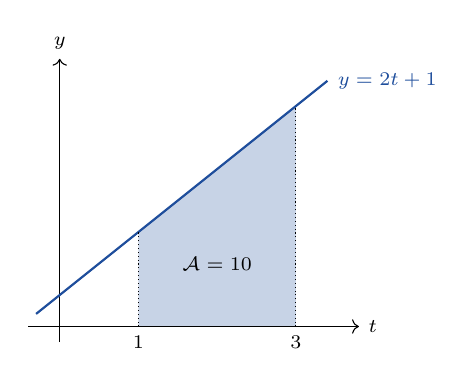
\begin{tikzpicture}[x=1cm,y=0.4cm,font=\scriptsize]
\fill[cDef!25] (1,0) -- (1,3) -- (3,7) -- (3,0) -- cycle;
\draw[->] (-0.4,0)--(3.8,0) node[right]{$t$}; \draw[->] (0,-0.5)--(0,8.5) node[above]{$y$};
\draw[cDef,thick] (-0.3,0.4)--(3.4,7.8) node[right]{$y=2t+1$};
\draw[densely dotted] (1,0)--(1,3) (3,0)--(3,7);
\node[below] at (1,0){$1$}; \node[below] at (3,0){$3$}; \node at (2,2){$\mathcal A=10$};
\end{tikzpicture}\end{LTR}\par \ck\ الحيز شبه منحرف: $\mathcal A=\dfrac{(3+7)\times2}2=10$.\par
\ck\ $F(t)=t^2+t$ دالة أصلية لـ $f$: $F(3)-F(1)=12-2=10$ ، نفس النتيجة.\par
}{35 د}{المقارنة بين الطريقتين.}
\Row{بناء المعارف}{%
\Lab{cDef}{تعريف}\ $f$ مستمرة على $I$ و $F$ دالة أصلية لها ، $a$ و $b$ من $I$: $\displaystyle\int_a^bf(t)\,dt=\big[F(t)\big]_a^b=F(b)-F(a)$.\par}{50 د}{دور المتغير الصامت.}
\Row{}{%
\Lab{cThm}{التفسير البياني}\ إذا كانت $f$ مستمرة وموجبة على $[a;b]$ ($a<b$) فإن $\displaystyle\int_a^bf(t)\,dt$ هو مساحة الحيز المحدد بـ $C_f$ ومحور الفواصل والمستقيمين $x=a$ و $x=b$ (بوحدة المساحات).\par}{}{}
\Row{}{%
\Lab{cEx}{مثال}\ $\displaystyle\int_0^2t^2\,dt=\left[\dfrac{t^3}3\right]_0^2=\dfrac83$.\par\smallskip\begin{LTR}\centering 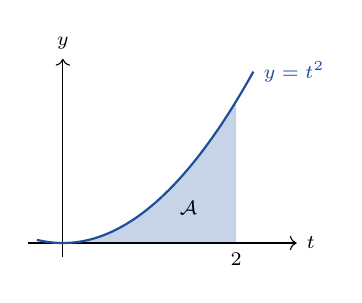
\begin{tikzpicture}[x=1.1cm,y=0.45cm,font=\scriptsize]
\fill[cDef!25] (0,0) -- plot[domain=0:2,samples=50] (\x,{\x*\x}) -- (2,0) -- cycle;
\draw[->] (-0.4,0)--(2.7,0) node[right]{$t$}; \draw[->] (0,-0.4)--(0,5.2) node[above]{$y$};
\draw[cDef,thick,domain=-0.3:2.2,samples=50] plot (\x,{\x*\x}) node[right]{$y=t^2$};
\node[below] at (2,0){$2$}; \node at (1.45,1){$\mathcal A$};
\end{tikzpicture}\end{LTR}\par }{}{}
\Row{}{%
\Lab{cRem}{ملاحظات}\ المتغير $t$ «صامت»: $\displaystyle\int_a^bf(t)\,dt=\int_a^bf(x)\,dx$.\par}{}{}
\Row{}{%
\Lab{cThm!80!black}{حذار}\ النتيجة لا تتعلق بالدالة الأصلية المختارة (الثابت يُختزل).}{}{}
\Row{التقويم}{%
\Lab{cEx}{تطبيق}\par احسب: $\displaystyle\int_1^2(3t^2-1)\,dt$ ؛ $\displaystyle\int_{-1}^1(t^3+2t)\,dt$. ثم: الكلفة الهامشية $C_m(q)=2q+10$: احسب $\displaystyle\int_0^{10}C_m(q)\,dq$ وفسّر.\par\textbf{الحل:} $\RR{6}$ \RR{؛} $\RR{0}$ \RR{؛} $\RR{\big[q^2+10q\big]_0^{10}=200}$: \RR{هو} $\RR{C(10)-C(0)}$ \RR{،} \RR{أي} \RR{زيادة} \RR{الكلفة} \RR{الإجمالية} \RR{لما} \RR{ننتج} $\RR{10}$ \RR{وحدات.}\par\textbf{واجب منزلي:} تمارين من باب التكامل.\par\smallskip\textbf{ملاحظات حول سير الحصة:} \dotfill}{25 د}{تقويم فردي.}
\end{Sayr}
\newpage
\ModhHead{25}{3 ت ا}{تحليل}{الدوال الأصلية والتكاملات}{02 سا}{خواص التكامل ، القيمة المتوسطة لدالة على مجال}%
{\begin{itemize}\item حساب التكامل.\end{itemize}}%
{\begin{itemize}\item توظيف خواص التكامل: الخطية ، علاقة شال ، الترتيب.\item حساب القيمة المتوسطة لدالة على مجال وتفسيرها.\end{itemize}}%
{المنهاج ، الكتاب المدرسي ، مراجع ، الحاسبة البيانية.}
\begin{Sayr}
\Row{مرحلة الانطلاق}{%
\textbf{التهيئة النفسية:} كيف نحسب متوسط كلفة هامشية تتغير مع الكمية بين $q=10$ و $q=20$ ؟}{10 د}{وضعية اقتصادية.}
\Row{التشخيص والاكتشاف}{%
\Lab{cEx}{وضعية مقترحة}\par\ck\ نحسب $\displaystyle\int_0^1x\,dx$ و $\displaystyle\int_0^1x^2\,dx$ ونقارن ، مع $x^2\leqslant x$ على $[0;1]$.\par
\ck\ نحسب $\displaystyle\int_0^3|x-1|\,dx$ بتقسيم المجال عند $1$.\par
}{35 د}{التحقق بالحساب.}
\Row{بناء المعارف}{%
\Lab{cThm}{خاصية}\par\ck\ $\displaystyle\int_a^af=0$ ؛ $\displaystyle\int_b^af=-\int_a^bf$.\par
\ck\ \textbf{الخطية}: $\displaystyle\int_a^b(\alpha f+\beta g)=\alpha\int_a^bf+\beta\int_a^bg$.\par
\ck\ \textbf{علاقة شال}: $\displaystyle\int_a^cf=\int_a^bf+\int_b^cf$.\par
\ck\ \textbf{الترتيب}: إذا كان $a\leqslant b$ و $f\leqslant g$ على $[a;b]$ فإن $\displaystyle\int_a^bf\leqslant\int_a^bg$ ؛ وإذا كانت $f\geqslant0$ فإن $\displaystyle\int_a^bf\geqslant0$.\par
}{50 د}{تفسير بياني بالمستطيل.}
\Row{}{%
\Lab{cEx}{مثال}\ $\dfrac13\leqslant\dfrac12$ ؛ $\displaystyle\int_0^3|x-1|\,dx=\int_0^1(1-x)\,dx+\int_1^3(x-1)\,dx=\dfrac12+2=\dfrac52$.\par}{}{}
\Row{}{%
\Lab{cDef}{القيمة المتوسطة}\ $\mu=\dfrac1{b-a}\displaystyle\int_a^bf(x)\,dx$ ؛ بيانياً: مساحة المستطيل الذي ارتفاعه $\mu$ تساوي مساحة الحيز تحت $C_f$.\par}{}{}
\Row{}{%
\Lab{cEx}{مثال}\ $C_m(q)=2q+10$ على $[10;20]$: $\mu=\dfrac1{10}\big[q^2+10q\big]_{10}^{20}=\dfrac{600-200}{10}=40$: متوسط الكلفة الهامشية.\par}{}{}
\Row{}{%
\Lab{cThm!80!black}{حذار}\ في الترتيب يجب $a\leqslant b$.}{}{}
\Row{التقويم}{%
\Lab{cEx}{تطبيق}\par $f(x)=3x^2-4x+1$. احسب $\displaystyle\int_0^2f(x)\,dx$ ثم القيمة المتوسطة لـ $f$ على $[0;2]$.\par\textbf{الحل:} $\RR{\big[x^3-2x^2+x\big]_0^2=2}$ \RR{؛} $\RR{\mu=\dfrac22=1}$.\par\textbf{واجب منزلي:} تمارين من باب التكامل (الخواص والقيمة المتوسطة).\par\smallskip\textbf{ملاحظات حول سير الحصة:} \dotfill}{25 د}{تقويم فردي.}
\end{Sayr}
\newpage
\ModhHead{26}{3 ت ا}{تحليل}{الدوال الأصلية والتكاملات}{02 سا}{حساب المساحات (1): الحيز بين منحنٍ ومحور الفواصل}%
{\begin{itemize}\item التكامل وخواصه ، إشارة دالة.\end{itemize}}%
{\begin{itemize}\item توظيف التكامل في حساب مساحة حيز محدد بمنحنٍ ومحور الفواصل.\end{itemize}}%
{المنهاج ، الكتاب المدرسي ، مراجع ، الحاسبة البيانية. ورق ميليمتري.}
\begin{Sayr}
\Row{مرحلة الانطلاق}{%
\textbf{التهيئة النفسية:} هل $\displaystyle\int_0^2(x^2-1)\,dx$ مساحة؟ احسبه وقارن بالرسم.}{10 د}{سؤال تحدٍّ.}
\Row{التشخيص والاكتشاف}{%
\Lab{cEx}{وضعية مقترحة}\ $f(x)=x^2-1$ على $[0;2]$: التكامل $\dfrac23$ ، لكن جزءاً من الحيز تحت محور الفواصل: التكامل «يطرح» ذلك الجزء.}{35 د}{جدول الإشارة قبل الحساب.}
\Row{بناء المعارف}{%
\Lab{cThm}{خاصية}\par\ck\ إذا كانت $f\geqslant0$ على $[a;b]$: $\mathcal A=\displaystyle\int_a^bf(x)\,dx$.\par
\ck\ إذا كانت $f\leqslant0$: $\mathcal A=-\displaystyle\int_a^bf(x)\,dx$.\par
\ck\ إذا تغيرت الإشارة نقسم المجال بعلاقة شال.\par
}{50 د}{تلوين كل حيز بلون.}
\Row{}{%
\Lab{cMeth}{طريقة}\ ندرس إشارة $f$ (الوضع النسبي لـ $C_f$ ومحور الفواصل) ، نرسم الحيز ، ثم نحسب. المساحة بوحدة المساحات $\text{u.a}$.\par}{}{}
\Row{}{%
\Lab{cEx}{مثال}\ $f(x)=x^2-1$ على $[0;2]$:\par\smallskip\begin{LTR}\centering {\footnotesize\renewcommand{\arraystretch}{1.45}\setlength{\tabcolsep}{2pt}\begin{tabular}{|>{\centering\arraybackslash}p{0.260\linewidth}|>{\centering\arraybackslash}p{0.120\linewidth}|>{\centering\arraybackslash}p{0.120\linewidth}|>{\centering\arraybackslash}p{0.120\linewidth}|>{\centering\arraybackslash}p{0.120\linewidth}|>{\centering\arraybackslash}p{0.120\linewidth}|}\hline\rowcolor{cSec!12}$x$ & $0$ &  & $1$ &  & $2$\\\hline$f(x)=x^2-1$ &  & $-$ & $0$ & $+$ & \\\hline\ar{الوضع النسبي} &  & \ar{$C_f$ تحت $(xx^{\prime})$} &  & \ar{$C_f$ فوق $(xx^{\prime})$} & \\\hline\end{tabular}}\end{LTR}\par \par\smallskip\begin{LTR}\centering 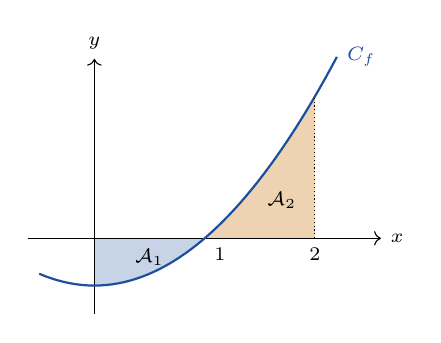
\begin{tikzpicture}[x=1.4cm,y=0.6cm,font=\scriptsize]
\fill[cDef!25] (0,0) -- plot[domain=0:1,samples=40] (\x,{\x*\x-1}) -- cycle;
\fill[cEx!30] (1,0) -- plot[domain=1:2,samples=40] (\x,{\x*\x-1}) -- (2,0) -- cycle;
\draw[->] (-0.6,0)--(2.6,0) node[right]{$x$}; \draw[->] (0,-1.6)--(0,3.8) node[above]{$y$};
\draw[cDef,thick,domain=-0.5:2.2,samples=50] plot (\x,{\x*\x-1}) node[right]{$C_f$};
\draw[densely dotted] (2,0)--(2,3);
\node[below right] at (1,0){$1$}; \node[below] at (2,0){$2$}; \node at (0.5,-0.4){$\mathcal A_1$}; \node at (1.7,0.8){$\mathcal A_2$};
\end{tikzpicture}\end{LTR}\par $\mathcal A_1=-\displaystyle\int_0^1(x^2-1)\,dx=\dfrac23$ ، $\mathcal A_2=\displaystyle\int_1^2(x^2-1)\,dx=\dfrac43$ ، $\mathcal A=2\ \text{u.a}$.\par}{}{}
\Row{}{%
\Lab{cThm!80!black}{حذار}\ إذا كانت الوحدة $\|\vec i\|=2\text{cm}$ و $\|\vec j\|=1\text{cm}$ فإن $1\ \text{u.a}=2\text{cm}^2$.}{}{}
\Row{التقويم}{%
\Lab{cEx}{تطبيق}\par احسب مساحة الحيز المحدد بمنحني $f(x)=-x^2+4x$ ومحور الفواصل والمستقيمين $x=0$ و $x=4$.\par\textbf{الحل:}\par\smallskip\begin{LTR}\centering {\footnotesize\renewcommand{\arraystretch}{1.45}\setlength{\tabcolsep}{2pt}\begin{tabular}{|>{\centering\arraybackslash}p{0.260\linewidth}|>{\centering\arraybackslash}p{0.200\linewidth}|>{\centering\arraybackslash}p{0.200\linewidth}|>{\centering\arraybackslash}p{0.200\linewidth}|}\hline\rowcolor{cSec!12}$x$ & $0$ &  & $4$\\\hline$f(x)=-x^2+4x$ & $0$ & $+$ & $0$\\\hline\ar{الوضع النسبي} &  & \ar{$C_f$ فوق $(xx^{\prime})$} & \\\hline\end{tabular}}\end{LTR}\par \par\smallskip\begin{LTR}\centering 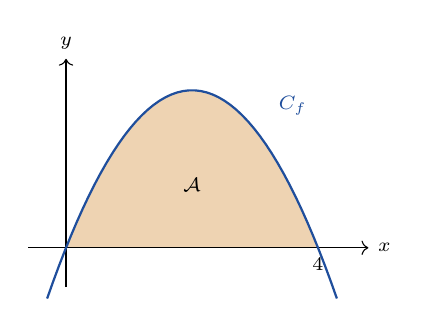
\begin{tikzpicture}[x=0.8cm,y=0.5cm,font=\scriptsize]
\fill[cEx!30] (0,0) -- plot[domain=0:4,samples=50] (\x,{-\x*\x+4*\x}) -- (4,0) -- cycle;
\draw[->] (-0.6,0)--(4.8,0) node[right]{$x$}; \draw[->] (0,-1)--(0,4.8) node[above]{$y$};
\draw[cDef,thick,domain=-0.3:4.3,samples=50] plot (\x,{-\x*\x+4*\x}); \node[cDef] at (3.6,3.6){$C_f$};
\node[below] at (4,0){$4$}; \node at (2,1.6){$\mathcal A$};
\end{tikzpicture}\end{LTR}\par $\RR{\mathcal A=\displaystyle\int_0^4(-x^2+4x)\,dx=\left[-\dfrac{x^3}3+2x^2\right]_0^4=\dfrac{32}3\ \text{u.a}}$.\par\textbf{واجب منزلي:} تمارين من باب التكامل (حساب المساحات).\par\smallskip\textbf{ملاحظات حول سير الحصة:} \dotfill}{25 د}{تقويم فردي.}
\end{Sayr}
\newpage
\ModhHead{27}{3 ت ا}{تحليل}{الدوال الأصلية والتكاملات}{02 سا}{حساب المساحات (2): الحيز بين منحنيين}%
{\begin{itemize}\item حساب المساحات ، الوضع النسبي لمنحنيين.\end{itemize}}%
{\begin{itemize}\item حساب مساحة حيز محدد بمنحنيين.\end{itemize}}%
{المنهاج ، الكتاب المدرسي ، مراجع ، الحاسبة البيانية. ورق ميليمتري.}
\begin{Sayr}
\Row{مرحلة الانطلاق}{%
\textbf{التهيئة النفسية:} كيف نحسب مساحة الحيز المحصور بين قطع مكافئ ومستقيم؟}{10 د}{سؤال.}
\Row{التشخيص والاكتشاف}{%
\Lab{cEx}{وضعية مقترحة}\ $f(x)=-x^2+4x$ و $g(x)=x$.\par\ck\ نقط التقاطع: $-x^2+4x=x$ يعطي $x=0$ أو $x=3$.\par
\ck\ المساحة بين المنحنيين = (المساحة تحت $C_f$) $-$ (المساحة تحت $C_g$).\par
}{35 د}{نقط التقاطع.}
\Row{بناء المعارف}{%
\Lab{cThm}{خاصية}\ إذا كان $f\geqslant g$ على $[a;b]$ فإن مساحة الحيز المحدد بـ $C_f$ و $C_g$ والمستقيمين $x=a$ و $x=b$ هي $\mathcal A=\displaystyle\int_a^b\big(f(x)-g(x)\big)\,dx$.\par}{50 د}{جدول الوضع النسبي والرسم.}
\Row{}{%
\Lab{cMeth}{طريقة}\ نعيّن نقط التقاطع ، ندرس إشارة $f-g$ (الوضع النسبي) ، نرسم الحيز ثم نحسب.\par}{}{}
\Row{}{%
\Lab{cEx}{مثال}\par\smallskip\begin{LTR}\centering {\footnotesize\renewcommand{\arraystretch}{1.45}\setlength{\tabcolsep}{2pt}\begin{tabular}{|>{\centering\arraybackslash}p{0.260\linewidth}|>{\centering\arraybackslash}p{0.200\linewidth}|>{\centering\arraybackslash}p{0.200\linewidth}|>{\centering\arraybackslash}p{0.200\linewidth}|}\hline\rowcolor{cSec!12}$x$ & $0$ &  & $3$\\\hline$f(x)-g(x)=-x^2+3x$ & $0$ & $+$ & $0$\\\hline\ar{الوضع النسبي} &  & \ar{$C_f$ فوق $C_g$} & \\\hline\end{tabular}}\end{LTR}\par \par\smallskip\begin{LTR}\centering 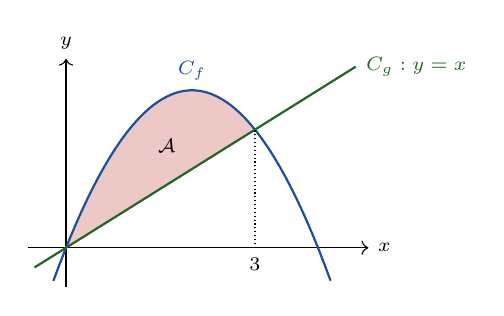
\begin{tikzpicture}[x=0.8cm,y=0.5cm,font=\scriptsize]
\fill[cThm!25] plot[domain=0:3,samples=50] (\x,{-\x*\x+4*\x}) -- plot[domain=3:0,samples=10] (\x,\x) -- cycle;
\draw[->] (-0.6,0)--(4.8,0) node[right]{$x$}; \draw[->] (0,-1)--(0,4.8) node[above]{$y$};
\draw[cDef,thick,domain=-0.2:4.2,samples=50] plot (\x,{-\x*\x+4*\x}); \node[cDef] at (2,4.5){$C_f$};
\draw[cRem!80!black,thick] (-0.5,-0.5)--(4.6,4.6) node[right]{$C_g:y=x$};
\draw[densely dotted] (3,0)--(3,3); \node[below] at (3,0){$3$}; \node at (1.6,2.6){$\mathcal A$};
\end{tikzpicture}\end{LTR}\par $\mathcal A=\displaystyle\int_0^3(-x^2+3x)\,dx=\left[-\dfrac{x^3}3+\dfrac32x^2\right]_0^3=\dfrac92\ \text{u.a}$.\par}{}{}
\Row{}{%
\Lab{cThm!80!black}{حذار}\ نطرح دائماً المنحني الأسفل من الأعلى.}{}{}
\Row{التقويم}{%
\Lab{cEx}{تطبيق}\par احسب مساحة الحيز المحصور بين المنحني $y=x^2$ والمستقيم $y=2x$.\par\textbf{الحل:} \RR{التقاطع} \RR{عند} $\RR{x=0}$ \RR{و} $\RR{x=2}$.\par\smallskip\begin{LTR}\centering {\footnotesize\renewcommand{\arraystretch}{1.45}\setlength{\tabcolsep}{2pt}\begin{tabular}{|>{\centering\arraybackslash}p{0.260\linewidth}|>{\centering\arraybackslash}p{0.200\linewidth}|>{\centering\arraybackslash}p{0.200\linewidth}|>{\centering\arraybackslash}p{0.200\linewidth}|}\hline\rowcolor{cSec!12}$x$ & $0$ &  & $2$\\\hline$2x-x^2$ & $0$ & $+$ & $0$\\\hline\ar{الوضع النسبي} &  & \ar{$y=2x$ \ar{فوق} $y=x^2$} & \\\hline\end{tabular}}\end{LTR}\par \par\smallskip\begin{LTR}\centering 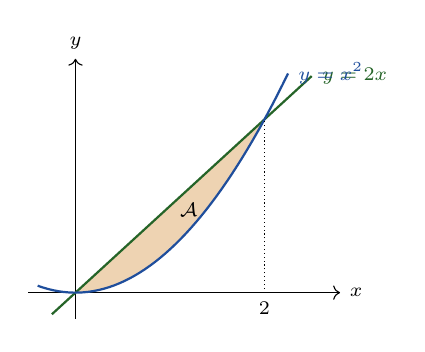
\begin{tikzpicture}[x=1.2cm,y=0.55cm,font=\scriptsize]
\fill[cEx!30] plot[domain=0:2,samples=10] (\x,{2*\x}) -- plot[domain=2:0,samples=40] (\x,{\x*\x}) -- cycle;
\draw[->] (-0.5,0)--(2.8,0) node[right]{$x$}; \draw[->] (0,-0.6)--(0,5.4) node[above]{$y$};
\draw[cRem!80!black,thick] (-0.25,-0.5)--(2.5,5) node[right]{$y=2x$};
\draw[cDef,thick,domain=-0.4:2.25,samples=50] plot (\x,{\x*\x}) node[right]{$y=x^2$};
\draw[densely dotted] (2,0)--(2,4); \node[below] at (2,0){$2$}; \node at (1.2,1.9){$\mathcal A$};
\end{tikzpicture}\end{LTR}\par $\RR{\mathcal A=\displaystyle\int_0^2(2x-x^2)\,dx=\left[x^2-\dfrac{x^3}3\right]_0^2=\dfrac43\ \text{u.a}}$.\par\textbf{واجب منزلي:} تمارين من باب التكامل (حساب المساحات).\par\smallskip\textbf{ملاحظات حول سير الحصة:} \dotfill}{25 د}{نهاية المحور: فرض أو مراجعة.}
\end{Sayr}
\end{document}
